%%%%%%%%%%%%%%%%%%%%%%%%%%%%%%%%%%%%%%%%%
% Propuesta de Desarrollo
% LaTeX Template
% Version 1.0 (06/02/2014)
%
% Original author:
% Federico Rossi (federicomrossi@gmail.com)
%
%%%%%%%%%%%%%%%%%%%%%%%%%%%%%%%%%%%%%%%%%



%------------------------------------------------------------------------------
%	PACKAGES AND OTHER DOCUMENT CONFIGURATIONS
%------------------------------------------------------------------------------

\documentclass{book}

% Paquetes generales
\usepackage[left=4cm, right=3cm, top=4cm, bottom=3cm, paperwidth=210mm, paperheight=297mm, headsep=1.5cm]{geometry}
\usepackage[utf8]{inputenc}
\usepackage[svgnames]{xcolor} % Required to specify font color
\usepackage{gensymb}

% Paquetes para estilos
\usepackage{textcomp}
\usepackage{setspace}
\usepackage{colortbl}
\usepackage{color}
\usepackage{color}
\usepackage{upquote}
\usepackage{xcolor}
\usepackage{listings}
\usepackage{caption}
\usepackage[T1]{fontenc}
\usepackage[scaled]{beramono}

% Paquetes extras
\usepackage{amssymb}
\usepackage{float}
\usepackage{graphicx}
\usepackage[export]{adjustbox}
\usepackage{url}
\usepackage[toc,page]{appendix}

% Paquete Matematica
\usepackage{mathtools}

% Paquetes para header y footer
\usepackage{fancyhdr}



% Definición de preferencias para la impresión de código fuente.
%% Colores
\definecolor{gray99}{gray}{.99}
\definecolor{gray95}{gray}{.95}
\definecolor{gray85}{gray}{.85}
\definecolor{gray75}{gray}{.75}
\definecolor{gray50}{gray}{.50}



\usepackage{titlesec}

\titleformat*{\section}{\LARGE\bfseries}
\titleformat*{\subsection}{\Large\bfseries}
\titleformat*{\subsubsection}{\large\bfseries}
\titleformat*{\paragraph}{\large\bfseries}
\titleformat*{\subparagraph}{\large\bfseries}

% Ocultamos numeración de las secciones
\setcounter{secnumdepth}{0}




%------------------------------------------------------------------------------
%	TITLE PAGE
%------------------------------------------------------------------------------

\newcommand*{\titleGM}{\begingroup % Create the command for including the title page in the document
\newcommand*{\sepline}{\color{gray85}\rule[0.5ex]{30em}{0.55pt}}
	
	% \hbox{ % Horizontal box
	% \hspace*{0.35\textwidth} % Whitespace to the left of the title page
	% %\rule{1pt}{\textheight} % Vertical line
	% \hspace*{0.05\textwidth} % Whitespace between the vertical line and title page text
	% \parbox[b]{0.75\textwidth}{ % Paragraph box which restricts text to less than the width of the page
	
	% % Logo luperosft
	% \begin{figure}[H]
	% \noindent\hspace*{0.0\textwidth}
	% 
\includegraphics[width=0.15\textwidth,left]{images/lupersoft-isotipo-fondo-blanco.png}
	% \end{figure}
	% \bigskip\bigskip

% \pagecolor{gray75}


% \vbox{
%     \begin{minipage}[t][0.5\textheight][t]{\textwidth}
%         Page 1
%     \end{minipage}

%     \nointerlineskip

%     \fboxsep0pt
%     \colorbox{green}{\begin{minipage}[b][0.5\textheight][t]{\textwidth}
    	
%         \vspace{0.4in}
%         Page 2
%     \end{minipage}}
% }


\begin{center}

	\vspace*{1.5cm} 
	
	% {\noindent\Huge\fontfamily{fvs}\selectfont SIGC \\[5\baselineskip]} % Title
	
\includegraphics[width=9cm]{images/graferator-logo.png} \\[12\baselineskip]

	
	\colorbox{gray95}{
		\parbox[t]{1.0\linewidth}{
			% \centering \fontsize{50pt}{80pt}\selectfont % The first argument for fontsize is the font size of the text and the second is the line spacing - you may need to play with these for your particular title
			\vspace*{0.7cm} % Space between the start of the title and the top of the grey box
			
			\centering {\Huge\bfseries\color{gray50}\fontfamily{fvs}\selectfont Guía de usuario}\par % Tagline or further description	
			
			\vspace*{0.7cm} % Space between the end of the title and the bottom of the grey box
		}
	}\\[10\baselineskip]


	% \sepline \\[1\baselineskip]
		\Large Belén Beltran \\
		\large \textit{belubeltran@gmail.com} \\ \medskip
		\Large Pablo Ariel Rodriguez \\
		\large \textit{prodriguez@fi.uba.ar} \\ \medskip
		\Large Federico Martin Rossi \\ 
		\large \textit{federicomrossi@gmail.com} \\

		\bigskip\bigskip\bigskip\bigskip

		\large 2do. Cuatrimestre 2014 \\ \smallskip
		\large 75.52 Taller de Programación II \\ \smallskip
		\large Facultad de Ingeniería, Universidad de Buenos Aires \\ \smallskip

\end{center}

	% }}
\endgroup}

\renewcommand{\chaptername}{Capítulo}
\renewcommand{\contentsname}{Contenido}
\titleformat{\chapter}[display]
  {\normalfont\bfseries\huge\color{black}}
  {\chaptertitlename\ \thechapter}{0.5em}{\textbf\Huge} 
\titleformat{\section}
  {\normalfont\Large\fontfamily{fvs}\bfseries\color{black}}
  {\thesection}{1em}{\Large}
\titleformat{\subsection}
  {\normalfont\Large\fontfamily{fvs}\color{cyan}}
  {\thesection}{1em}{\Large}

% \titleformat{\chapter}[hang] 
% {\normalfont\Huge\fontfamily{fvs}}{\chaptertitlename\ \thechapter:}{0.5em}{\Huge} 
% \titleformat{\section}{\normalfont\Large\fontfamily{fvs}}{\thesection}{1em}{\Large}


%% FIGURAS
\captionsetup[figure]{labelfont=bf,textfont=it}
%% TABLAS
\captionsetup[table]{labelfont=bf,textfont=it}

% COMANDOS

%% Titulo de las cajas de código
\renewcommand{\lstlistingname}{Código}
%% Titulo de las figuras
\renewcommand{\figurename}{Imagen}
%% Titulo de las tablas
\renewcommand{\tablename}{Tabla}
%% Referencia a los códigos
\newcommand{\refcode}[1]{\textit{Código \ref{#1}}}
%% Referencia a las imagenes
\newcommand{\refimage}[1]{\textit{Imagen \ref{#1}}}




%------------------------------------------------------------------------------
%	HEADER AND FOOTER
%------------------------------------------------------------------------------


% \pagestyle{fancy}

% \lhead{SIGC}
% \chead{Guía de Usuario}
% \rhead{
\includegraphics[width=0.4cm]{images/lupersoft-isotipo.png}}
% \lfoot{}
% \cfoot{}
% \rfoot{}




%------------------------------------------------------------------------------
%	BLANK DOCUMENT
%------------------------------------------------------------------------------

\begin{document}

\pagenumbering{roman}
% \setcounter{page}{0}

% \pagestyle{empty} % Removes page numbers
\thispagestyle{empty}


% This command includes the title page
\titleGM
% \thispagestyle{empty}
% \newpage \textit{}
% \thispagestyle{empty}
% \newpage \textit{}
% \thispagestyle{empty}



%
% TEXTOS PREVIOS
%
\section*{\bfseries\color{black}Antes de empezar}

Esta guía asume que el lector se encuentra familiarizado con el sistema operativo \textit{Microsoft Windows} (versión XP y posteriores) y aquellos basados en GNU/Linux. Es decir, se considera que el usuario se encuentra mínimamente en condiciones de desenvolverse en el entorno en el cual se ejecuta la aplicación, razón por la cual no se explican temas como la utilización de cuadros de diálogo, asistentes, el exploradores de carpetas o el uso de la consola de comandos.
\bigskip


\section*{Objetivo}

El objetivo principal de esta guía es ayudar y guiar al usuario en la instalación, así como también en la utilización de \textbf{Graferator} haciendo hincapié en las características y opciones más relevantes que se presentan en este. 
\bigskip


\section*{\bfseries\color{black}Cómo leer esta guía}

Se recomienda al usuario leer esta guía teniendo a la vista de su pantalla el software ejecutándose. Esto le permitirá poder realizar los pasos aquí detallados a medida que avanza en la lectura, logrando asimilar más fácilmente la disposición de las distintas opciones mencionadas y la forma en que estas deben ser utilizadas.
\bigskip


\section*{\bfseries\color{black}Organización}

La guía está compuesta de capítulos que agrupan las distintas funcionalidades provistas por la aplicación y que se encuentran relacionadas entre sí. Las secciónes que conforman los capítulos detallan los pasos a seguir para poder hacer uso de dichas funcionalidades.



% ÍNDICE
\tableofcontents
\newpage
\thispagestyle{empty}
\pagenumbering{arabic}
\thispagestyle{empty}
\thispagestyle{empty}




%
% CAPITULO 1
%
\chapter{Instalación}


% CAPITULO 1
% Requerimientos de hardware
\section{Requerimientos de hardware}

	Asegúrese de que su equipo cumple con los requerimientos mínimos de hardware:
	\medskip

	\begin{itemize}
		\renewcommand{\labelitemi}{\scriptsize\tiny$\blacksquare$} 
		\itemsep=5pt \topsep=0pt \partopsep=0pt \parskip=0pt \parsep=0pt

		\item \textit{Memoria RAM}: 128MB mínimo, 512MB recomendado;
		\item \textit{Espacio en disco}: 30MB para Graferator; 124 MB para JRE; 2 MB para Java Update; 
		\item \textit{Procesador}: Mínimo Pentium 2 a 266 MHz;

	\end{itemize}
\bigskip


% CAPITULO 1
% Requerimientos de software
\section{Requerimientos de software}

Asegúrese de que su sistema cumple los requisitos de software mínimos recomendados, los cuales se encuentran especificados a continuación:
	\medskip

	\begin{itemize}
		\renewcommand{\labelitemi}{\scriptsize\tiny$\blacksquare$} 
		\itemsep=5pt \topsep=0pt \partopsep=0pt \parskip=0pt \parsep=0pt

		\item \textit{Sistemas operativos}: GNU/Linux (x86 y x86-64) con interfaz gráfica; Windows 8 (escritorio), Windows 7, Windows Vista SP2;

		\item \textit{Java Runtime Enviroment} (JRE o JVM) (\url{http://java.com});

		\item Descompresor de archivos con formato \textit{ZIP}. (e.g.: WinZIP en Microsoft Windows).

	\end{itemize}
\bigskip



% CAPITULO 1
% Instalación del software en Microsoft Windows
\section{Instalación en Microsoft Windows}

\begin{enumerate}
	\itemsep=8pt \topsep=0pt \partopsep=0pt \parskip=0pt \parsep=0pt
	
	\item \textbf{Cree una nueva carpeta} con el nombre \textit{Graferator} en alguna ubicación de su preferencia (por lo general las instalaciones se realizan sobre el directorio C:\\Archivos de programas);

	\item \textbf{Sitúe el archivo} \textit{Graferator-version-X.zip} en la carpeta que ha creado. \textit{Nota: reemplace X por el número de versión que se encuentra instalando; por ejemplo, para la versión 1.0 el archivo se llamará Graferator-version-1.0.zip};

	\item \textbf{Descomprima} el archivo Zip asegurándose de que el archivo con extensión .jar \textit{Graferator.jar} se mantenga en la raíz del directorio creado en el primer paso;

	\item \textbf{Haga doble click} sobre el archivo \textit{Graferator.jar} para ejecutar Graferator.

	\item Si lo desea, puede \textbf{ejecutar} Graferator desde la \textbf{línea de comandos (consola)} posicionándose con esta última sobre la carpeta donde se encuentra el archivo \textit{Graferator.jar} y ejecutando la línea ``{\ttfamily\footnotesize java -jar graferator.jar}''

\end{enumerate}
\bigskip



% CAPITULO 1
% Instalación del software en SO basados en GNU/Linux
\section{Instalación en SO basados en GNU/Linux}

\begin{enumerate}
	\itemsep=8pt \topsep=0pt \partopsep=0pt \parskip=0pt \parsep=0pt
	
	\item \textbf{Cree una nueva carpeta} con el nombre \textit{Graferator} en alguna ubicación de su preferencia (por lo general las instalaciones se realizan sobre el directorio /usr/bin );

	\item \textbf{Sitúe el archivo} \textit{Graferator-version-X.zip} en la carpeta que ha creado. \textit{Nota: reemplace X por el número de versión que se encuentra instalando; por ejemplo, para la versión 1.0 el archivo se llamará Graferator-version-1.0.zip};

	\item \textbf{Descomprima} el archivo Zip asegurándose de que el archivo con extensión .jar \textit{Graferator.jar} se mantenga en la raíz del directorio creado en el primer paso. Por lo general se suele descomprimir utilizando el comando ``{\ttfamily\footnotesize \$ unzip Graferator-version-X.zip}''

	\item \textbf{Ejecute} Graferator desde la \textbf{línea de comandos (consola)} posicionándose con esta última sobre la carpeta donde se encuentra el archivo \textit{Graferator.jar} y ejecute la línea ``{\ttfamily\footnotesize \$ java -jar graferator.jar}''.

\end{enumerate}
\bigskip




%
% CAPITULO 2
%
\chapter{Primeros pasos}


% CAPITULO 2
% Espacio de trabajo
\section{Espacio de trabajo}

Una vez iniciada la aplicación se abrirá la ventana principal de Graferator, en donde se encuentra el espacio de trabajo sobre el cual podrá desenvolverse el usuario. En la \textit{Imagen 2.1} se puede observar el entorno completo.
\bigskip

% Imagen Ventana 01
\begin{figure}[H]
	\centering
	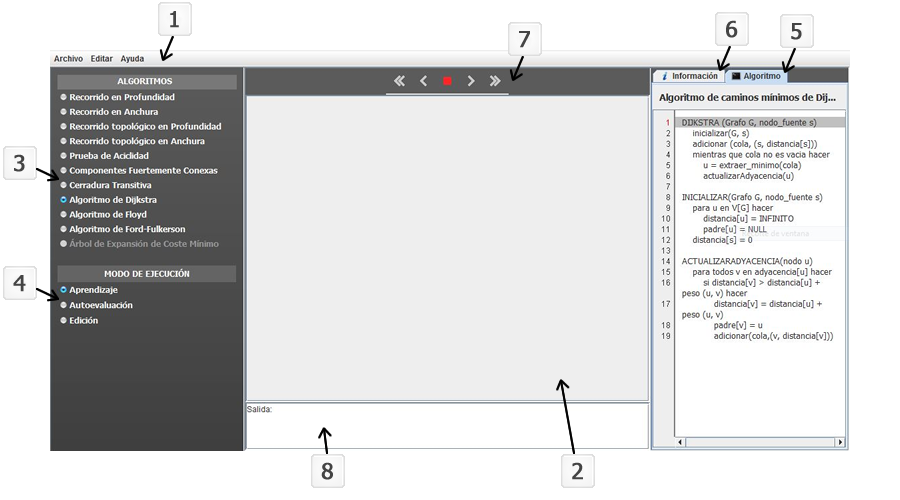
\includegraphics[width=1.0\textwidth]{images/ventanas/01.png}
	\caption{Espacio de trabajo de Graferator.}
\end{figure}
\bigskip


Tomando como referencia la \textit{Imagen 2.1}, el espacio de trabajo está conformado por las siguientes características:

\begin{enumerate}
	\itemsep=8pt \topsep=0pt \partopsep=0pt \parskip=0pt \parsep=0pt
	
	\item [] 
\includegraphics[width=0.5cm]{images/number-1.png} \textbf{Menú}: contiene las opciones principales, entre ellas, \textit{Nuevo} (permite crear un nuevo grafo), \textit{Editar} (contiene opciones que permiten agregar vértices y aristas);

	\item [] 
\includegraphics[width=0.5cm]{images/number-2.png} \textbf{Área de diseño}: zona en donde se creará el grafo a través de la disposición de vértices sobre dicho espacio;

	\item [] 
\includegraphics[width=0.5cm]{images/number-3.png} \textbf{Algoritmos}: listado de algoritmos aplicables al grafo. Aparecerán habilitados o deshabilitados dependiendo de si es posible ejecutar el algoritmo sobre el grafo existente en el área de diseño;

	\item [] 
\includegraphics[width=0.5cm]{images/number-4.png} \textbf{Modos de ejecución}: permite elegir entre tres modos, \textit{Modo Edición} (instancia en la que se habilita la edición del grafo sobre el área de diseño), \textit{Modo Aprendizaje} (ejecuta el algoritmo paso a paso sobre el grafo) y \textit{Modo Autoevaluación} (el usuario es evaluado para corroborar que posee conocimiento de cómo se ejecuta el algoritmo activo);

	\item [] 
\includegraphics[width=0.5cm]{images/number-5.png} \textbf{Algoritmo}: pestaña en donde se visualizan los distintos pseudocódigos. Las líneas de estos serán resaltadas en concordancia con el avance del algoritmo;

	\item [] 
\includegraphics[width=0.5cm]{images/number-6.png} \textbf{Información}: pestaña en donde se visualiza la información general del algoritmo activo;

	\item [] 
\includegraphics[width=0.5cm]{images/number-7.png} \textbf{Controles de ejecución}: controles con los que iniciar y detener la ejecución del algoritmo. Además, cuenta con botones para avanzar o retroceder paso a paso, así como también ir directamente al final o al inicio del proceso;

	\item [] 
\includegraphics[width=0.5cm]{images/number-8.png} \textbf{Salida}: panel en donde se muestra la salida de cada algoritmo, es decir, resultados entre otros mensajes posibles;

\end{enumerate}
\medskip





% CAPITULO 2
% Crear nuevo grafo
\section{Crear nuevo grafo}

Para crear un nuevo grafo, siga los siguientes pasos:
\medskip

\begin{enumerate}
	\itemsep=8pt \topsep=0pt \partopsep=0pt \parskip=0pt \parsep=0pt
	
	\item Diríjase con el puntero del mouse hacia la barra de menú superior y \textbf{haga click} sobre la opción \textbf{Archivo}.

	\item \textbf{Seleccione} la opción \textbf{Nuevo}.

	\item \textbf{Elija} si desea crear un \textbf{Grafo Orientado} o un \textbf{Grafo No Orientado} (\textit{Imagen 2.2}).

	\item Para cualquiera de los tipos de grafo elegido, \textbf{seleccione} si desea un \textbf{Grafo vacío} o un \textbf{Grafo aleatorio}.

	\item  En caso de elegir un grafo vacío, se abrirá un proyecto nuevo con el área de diseño vacía.

	\item Si se ha elegido un grafo aleatorio, aparecerá una ventana emergente en la que se le solicitará que \textbf{ingrese} la \textbf{ cantidad de vértices} y la \textbf{cantidad de aristas}. Una vez hecho esto \textbf{presione} el botón \textbf{Aceptar} para cargar el nuevo grafo sobre el área de diseño.

\end{enumerate}
\smallskip


% CAPITULO 2
% Abrir grafo existente
\section{Abrir grafo existente}

Para abrir un grafo ya creado y almacenado en su computadora, siga los siguientes pasos:
\medskip

\begin{enumerate}
	\itemsep=8pt \topsep=0pt \partopsep=0pt \parskip=0pt \parsep=0pt

	\item Diríjase con el puntero del mouse hacia la barra de menú superior y \textbf{haga click} sobre la opción \textbf{Archivo}.

	\item \textbf{Seleccione} la opción \textbf{Abrir}. Se abrirá una ventana emergente.

	\item \textbf{Busque} el \textbf{archivo de extensión .gpht} a través del explorador de la ventana y \textbf{seleccionelo}.

	\item \textbf{Haga click} sobre el botón \textbf{Abrir}.

	\item Se cargará el grafo sobre el área de trabajo.

\end{enumerate}
\medskip


% Imagen Ventana 02
\begin{figure}[H]
	\centering
	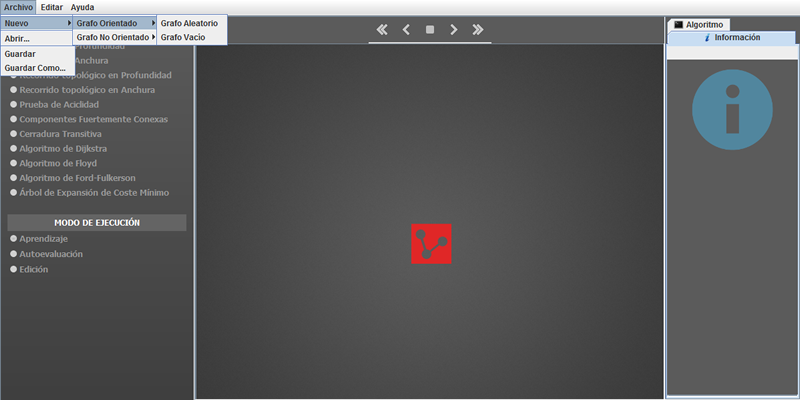
\includegraphics[width=1.0\textwidth]{images/ventanas/02.png}
	\medskip
	\caption{Menú para la creación de un grafo nuevo.}
\end{figure}
\bigskip



% CAPITULO 2
% Guardar grafo
\section{Guardar grafo}

Para guardar el grafo actualmente activo sobre el área de diseño, siga los siguientes pasos:
\medskip

\begin{enumerate}
	\itemsep=8pt \topsep=0pt \partopsep=0pt \parskip=0pt \parsep=0pt

	\item Diríjase con el puntero del mouse hacia la barra de menú superior y \textbf{haga click} sobre la opción \textbf{Archivo}.

	\item \textbf{Seleccione} la opción \textbf{Guardar Como...}. Se abrirá una ventana emergente.

	\item \textbf{Posicionese} en el directorio sobre el cual desea guardar el archivo.

	\item \textbf{Escriba} un \textbf{nombre de archivo} con el cual desea reconocer a este último.

	\item \textbf{Haga click} sobre el botón \textbf{Guardar} ubicado en la esquina inferior derecha de la ventana.

\end{enumerate}
\medskip


Una vez guardado inicialmente el grafo, usted puede guardar cualquier cambio que se produzca en adelante realizando los siguientes pasos:

\begin{enumerate}
	\itemsep=8pt \topsep=0pt \partopsep=0pt \parskip=0pt \parsep=0pt

	\item Diríjase con el puntero del mouse hacia la barra de menú superior y \textbf{haga click} sobre la opción \textbf{Archivo}.

	\item \textbf{Seleccione} la opción \textbf{Guardar}.

	\item Automáticamente se guardarán los cambios sobre el último archivo abierto o guardado.

\end{enumerate}
\medskip




%
% CAPITULO 3
%
\chapter{Armado de grafos}

% Agregar vértice
\section{Agregar vértice}

Para agregar un nuevo vértice al grafo, realice los siguientes pasos:
\medskip

\begin{enumerate}
	\itemsep=8pt \topsep=0pt \partopsep=0pt \parskip=0pt \parsep=0pt

	\item Diríjase con el puntero del mouse hacia la barra de menú superior y \textbf{haga click} sobre la opción \textbf{Editar}.

	\item \textbf{Seleccione} la opción \textbf{Nuevo vértice}.

	\item Aparecerá un vértice cuyo nombre será ``vN'', siendo N un número natural. Este nombre será la identificación del vértice.

\end{enumerate}
\medskip

Además, puede agregar un vértice de una forma mas simple \textbf{haciendo doble click} sobre el área de diseño.
\bigskip


% Imagen Ventana 02
\begin{figure}[H]
	\centering
	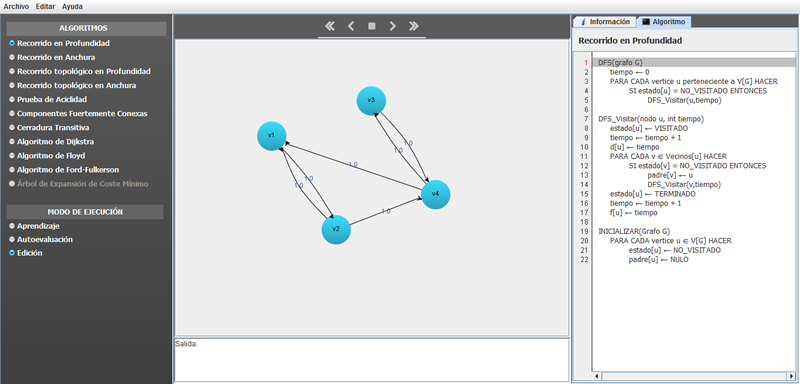
\includegraphics[width=1.0\textwidth]{images/ventanas/03.png}
	\medskip
	\caption{Ejemplo de grafo armado sobre el área de diseño.}
\end{figure}
\bigskip



% Eliminar vértice
\section{Eliminar vértice}

Para eliminar un vértice del grafo, realice los siguientes pasos:
\medskip

\begin{enumerate}
	\itemsep=8pt \topsep=0pt \partopsep=0pt \parskip=0pt \parsep=0pt

	\item \textbf{Haga click} sobre el vértice que desea eliminar. Esto hará que quede seleccionado.

	\item \textbf{Presione} la tecla \textbf{Supr} o \textbf{Del} para quitar el vértice y las aristas que lo relacionan con otros vértices.

\end{enumerate}
\medskip



% Agregar arista
\section{Agregar arista}

Para agregar una nueva arista al grafo, realice los siguientes pasos:
\medskip

\begin{enumerate}
	\itemsep=8pt \topsep=0pt \partopsep=0pt \parskip=0pt \parsep=0pt

	\item Diríjase con el puntero del mouse hacia la barra de menú superior y \textbf{haga click} sobre la opción \textbf{Editar}.

	\item \textbf{Seleccione} la opción \textbf{Nueva arista}.

	\item Se abrirá una ventana sobre la cual debe especificar el nombre del vértice de origen, el nombre del vértice destino y el peso o ponderación que tendrá esta.

	\item \textbf{Haga click} sobre el botón \textbf{Aceptar} para concretar la creación de la arista.

\end{enumerate}
\medskip

Además, puede agregar un arista de una forma mas simple y directa \textbf{haciendo click} con el \textbf{botón izquierdo del mouse} sobre el vértice origen y, sin soltarlo, arrastrar el puntero hasta posicionarlo sobre el vértice destino. Una vez allí deberá \textbf{soltar el botón del mouse}. Se creará así una arista de peso 1, el cual puede ser modificado haciéndole \textbf{doble click} encima de la ponderación y tipeando el nuevo valor a asignarle.
\medskip


% Eliminar arista
\section{Eliminar arista}

Para eliminar una arista del grafo, realice los siguientes pasos:
\medskip

\begin{enumerate}
	\itemsep=8pt \topsep=0pt \partopsep=0pt \parskip=0pt \parsep=0pt

	\item \textbf{Haga click} sobre la arista que desea eliminar. Esto hará que quede seleccionada.

	\item \textbf{Presione} la tecla \textbf{Supr} o \textbf{Del} para quitar la arista.

\end{enumerate}
\medskip




%
% CAPITULO 4
%
\chapter{Algoritmo de Recorrido en Profundidad}


% Ejecución en Modo Aprendizaje
\section{Ejecución en Modo Aprendizaje}

Para ejecutar el algoritmo en modo aprendizaje sobre el grafo existente en la zona de trabajo, realice los siguientes pasos:
\medskip

\begin{enumerate}
	\itemsep=8pt \topsep=0pt \partopsep=0pt \parskip=0pt \parsep=0pt

	\item \textbf{Haga click} sobre la opción \textbf{Aprendizaje} del panel de \textbf{Modo de Ejecución};

	\item \textbf{Haga click} sobre la opción \textbf{Recorrido en Profundidad} del panel de \textbf{Algoritmos};

	\item \textbf{Haga click} sobre el \textbf{vértice} que desee sea considerado el \textbf{vértice origen}. Deberá aparecer un cuadro de diálogo que indicará que el vértice de origen fue elgido;

	\item Inicie la ejecución \textbf{haciendo Click} sobre el botón \textbf{Comenzar/Finalizar} de la barra de \textbf{Controles de ejecución} ubicado en la parte superior de la ventana;

	\item Avance sobre el algoritmo \textbf{haciendo click} sobre el botón \textbf{Avanzar} ubicado a la derecha del botón \textit{Comenzar} de la barra de \textbf{Controles de ejecución};

	\item A medida que avance verá que los vértices se irán iluminando indicando el recorrido sobre el grafo. Verá sobre el panel de \textbf{Salida} la secuencia del recorrido;

	\item \textbf{Haga click} sobre el botón \textbf{Fin} de la barra de \textbf{Controles de ejecución} para ir directamente al \textbf{final del algoritmo}. Sobre el panel de \textbf{Salida} verá la secuencia final del recorrido;

	\item Detenga la ejecución \textbf{haciendo Click} sobre el botón \textbf{Comenzar/Finalizar} de la barra de \textbf{Controles de ejecución}.

\end{enumerate}
\medskip



% Ejecución en Modo Autoevaluación
\section{Ejecución en Modo Autoevaluación}

Para ejecutar el algoritmo en modo autoevaluación sobre el grafo existente en la zona de trabajo, realice los siguientes pasos:
\medskip

\begin{enumerate}
	\itemsep=8pt \topsep=0pt \partopsep=0pt \parskip=0pt \parsep=0pt

	\item \textbf{Haga click} sobre la opción \textbf{Autoevaluacíón} del panel de \textbf{Modo de Ejecución};

	\item \textbf{Haga click} sobre la opción \textbf{Recorrido en Profundidad} del panel de \textbf{Algoritmos};

	\item \textbf{Haga click} sobre el \textbf{vértice} que desee sea considerado el \textbf{vértice origen}. Deberá aparecer un cuadro de diálogo que indicará que el vértice de origen fue elgido;

	\item Inicie la ejecución \textbf{haciendo Click} sobre el botón \textbf{Comenzar/Finalizar} de la barra de \textbf{Controles de ejecución} ubicado en la parte superior de la ventana;

	\item \textbf{Haga click} sobre el vértice que cree que será elegido por el algoritmo en el paso siguiente.

	\item Avance sobre el algoritmo \textbf{haciendo click} sobre el botón \textbf{Avanzar} ubicado a la derecha del botón \textit{Comenzar} de la barra de \textbf{Controles de ejecución}. Si el vértice que ha elegido es el correcto, verá un mensaje que así lo indique. De lo contrario, se le indicará que la elección fue incorrecta y deberá volver a elegir un nuevo vértice, para luego volver a intentar pasar al siguiente paso del algoritmo;

	\item Detenga la ejecución \textbf{haciendo Click} sobre el botón \textbf{Comenzar/Finalizar} de la barra de \textbf{Controles de ejecución}.

\end{enumerate}
\medskip



%
% CAPITULO 5
%
\chapter{Algoritmo de Recorrido en Anchura}


% Ejecución en Modo Aprendizaje
\section{Ejecución en Modo Aprendizaje}

Para ejecutar el algoritmo en modo aprendizaje sobre el grafo existente en la zona de trabajo, realice los siguientes pasos:
\medskip

\begin{enumerate}
	\itemsep=8pt \topsep=0pt \partopsep=0pt \parskip=0pt \parsep=0pt

	\item \textbf{Haga click} sobre la opción \textbf{Aprendizaje} del panel de \textbf{Modo de Ejecución};

	\item \textbf{Haga click} sobre la opción \textbf{Recorrido en Anchura} del panel de \textbf{Algoritmos};

	\item \textbf{Haga click} sobre el \textbf{vértice} que desee sea considerado el \textbf{vértice origen}. Deberá aparecer un cuadro de diálogo que indicará que el vértice de origen fue elgido;

	\item Inicie la ejecución \textbf{haciendo Click} sobre el botón \textbf{Comenzar/Finalizar} de la barra de \textbf{Controles de ejecución} ubicado en la parte superior de la ventana;

	\item Avance sobre el algoritmo \textbf{haciendo click} sobre el botón \textbf{Avanzar} ubicado a la derecha del botón \textit{Comenzar} de la barra de \textbf{Controles de ejecución};

	\item A medida que avance verá que los vértices se irán iluminando indicando el recorrido sobre el grafo. Verá sobre el panel de \textbf{Salida} la secuencia del recorrido;

	\item \textbf{Haga click} sobre el botón \textbf{Fin} de la barra de \textbf{Controles de ejecución} para ir directamente al \textbf{final del algoritmo}. Sobre el panel de \textbf{Salida} verá la secuencia final del recorrido;

	\item Detenga la ejecución \textbf{haciendo Click} sobre el botón \textbf{Comenzar/Finalizar} de la barra de \textbf{Controles de ejecución}.

\end{enumerate}
\medskip



% Ejecución en Modo Autoevaluación
\section{Ejecución en Modo Autoevaluación}

Para ejecutar el algoritmo en modo autoevaluación sobre el grafo existente en la zona de trabajo, realice los siguientes pasos:
\medskip

\begin{enumerate}
	\itemsep=8pt \topsep=0pt \partopsep=0pt \parskip=0pt \parsep=0pt

	\item \textbf{Haga click} sobre la opción \textbf{Autoevaluacíón} del panel de \textbf{Modo de Ejecución};

	\item \textbf{Haga click} sobre la opción \textbf{Recorrido en Anchura} del panel de \textbf{Algoritmos};

	\item \textbf{Haga click} sobre el \textbf{vértice} que desee sea considerado el \textbf{vértice origen}. Deberá aparecer un cuadro de diálogo que indicará que el vértice de origen fue elgido;

	\item Inicie la ejecución \textbf{haciendo Click} sobre el botón \textbf{Comenzar/Finalizar} de la barra de \textbf{Controles de ejecución} ubicado en la parte superior de la ventana;

	\item \textbf{Haga click} sobre el vértice que cree que será elegido por el algoritmo en el paso siguiente.

	\item Avance sobre el algoritmo \textbf{haciendo click} sobre el botón \textbf{Avanzar} ubicado a la derecha del botón \textit{Comenzar} de la barra de \textbf{Controles de ejecución}. Si el vértice que ha elegido es el correcto, verá un mensaje que así lo indique. De lo contrario, se le indicará que la elección fue incorrecta y deberá volver a elegir un nuevo vértice, para luego volver a intentar pasar al siguiente paso del algoritmo;

	\item Detenga la ejecución \textbf{haciendo Click} sobre el botón \textbf{Comenzar/Finalizar} de la barra de \textbf{Controles de ejecución}.

\end{enumerate}
\medskip



%
% CAPITULO 6
%
\chapter{Algoritmo de Recorrido topológico en Profundidad}


% Ejecución en Modo Aprendizaje
\section{Ejecución en Modo Aprendizaje}

Para ejecutar el algoritmo en modo aprendizaje sobre el grafo existente en la zona de trabajo, realice los siguientes pasos:
\medskip

\begin{enumerate}
	\itemsep=8pt \topsep=0pt \partopsep=0pt \parskip=0pt \parsep=0pt

	\item \textbf{Haga click} sobre la opción \textbf{Aprendizaje} del panel de \textbf{Modo de Ejecución};

	\item \textbf{Haga click} sobre la opción \textbf{Recorrido topológico en Profundidad} del panel de \textbf{Algoritmos};

	\item Inicie la ejecución \textbf{haciendo Click} sobre el botón \textbf{Comenzar/Finalizar} de la barra de \textbf{Controles de ejecución} ubicado en la parte superior de la ventana;

	\item Avance sobre el algoritmo \textbf{haciendo click} sobre el botón \textbf{Avanzar} ubicado a la derecha del botón \textit{Comenzar} de la barra de \textbf{Controles de ejecución};

	\item A medida que avance verá que los vértices se irán iluminando indicando el recorrido sobre el grafo. Verá sobre el panel de \textbf{Salida} la secuencia del recorrido;

	\item \textbf{Haga click} sobre el botón \textbf{Fin} de la barra de \textbf{Controles de ejecución} para ir directamente al \textbf{final del algoritmo}. Sobre el panel de \textbf{Salida} verá la secuencia final del recorrido;

	\item Detenga la ejecución \textbf{haciendo Click} sobre el botón \textbf{Comenzar/Finalizar} de la barra de \textbf{Controles de ejecución}.

\end{enumerate}
\medskip



% Ejecución en Modo Autoevaluación
\section{Ejecución en Modo Autoevaluación}

Para ejecutar el algoritmo en modo autoevaluación sobre el grafo existente en la zona de trabajo, realice los siguientes pasos:
\medskip

\begin{enumerate}
	\itemsep=8pt \topsep=0pt \partopsep=0pt \parskip=0pt \parsep=0pt

	\item \textbf{Haga click} sobre la opción \textbf{Autoevaluacíón} del panel de \textbf{Modo de Ejecución};

	\item \textbf{Haga click} sobre la opción \textbf{Recorrido topológico en Profundidad} del panel de \textbf{Algoritmos};

	\item Inicie la ejecución \textbf{haciendo Click} sobre el botón \textbf{Comenzar/Finalizar} de la barra de \textbf{Controles de ejecución} ubicado en la parte superior de la ventana;

	\item \textbf{Haga click} sobre el vértice que cree que será elegido por el algoritmo en el paso siguiente.

	\item Avance sobre el algoritmo \textbf{haciendo click} sobre el botón \textbf{Avanzar} ubicado a la derecha del botón \textit{Comenzar} de la barra de \textbf{Controles de ejecución}. Si el vértice que ha elegido es el correcto, verá un mensaje que así lo indique. De lo contrario, se le indicará que la elección fue incorrecta y deberá volver a elegir un nuevo vértice, para luego volver a intentar pasar al siguiente paso del algoritmo;

	\item Detenga la ejecución \textbf{haciendo Click} sobre el botón \textbf{Comenzar/Finalizar} de la barra de \textbf{Controles de ejecución}.

\end{enumerate}
\medskip




%
% CAPITULO 7
%
\chapter{Algoritmo de Recorrido topológico en Anchura}


% Ejecución en Modo Aprendizaje
\section{Ejecución en Modo Aprendizaje}

Para ejecutar el algoritmo en modo aprendizaje sobre el grafo existente en la zona de trabajo, realice los siguientes pasos:
\medskip

\begin{enumerate}
	\itemsep=8pt \topsep=0pt \partopsep=0pt \parskip=0pt \parsep=0pt

	\item \textbf{Haga click} sobre la opción \textbf{Aprendizaje} del panel de \textbf{Modo de Ejecución};

	\item \textbf{Haga click} sobre la opción \textbf{Recorrido topológico en Anchura} del panel de \textbf{Algoritmos};

	\item Inicie la ejecución \textbf{haciendo Click} sobre el botón \textbf{Comenzar/Finalizar} de la barra de \textbf{Controles de ejecución} ubicado en la parte superior de la ventana;

	\item Avance sobre el algoritmo \textbf{haciendo click} sobre el botón \textbf{Avanzar} ubicado a la derecha del botón \textit{Comenzar} de la barra de \textbf{Controles de ejecución};

	\item A medida que avance verá que los vértices se irán iluminando indicando el recorrido sobre el grafo. Verá sobre el panel de \textbf{Salida} la secuencia del recorrido;

	\item \textbf{Haga click} sobre el botón \textbf{Fin} de la barra de \textbf{Controles de ejecución} para ir directamente al \textbf{final del algoritmo}. Sobre el panel de \textbf{Salida} verá la secuencia final del recorrido;

	\item Detenga la ejecución \textbf{haciendo Click} sobre el botón \textbf{Comenzar/Finalizar} de la barra de \textbf{Controles de ejecución}.

\end{enumerate}
\medskip



% Ejecución en Modo Autoevaluación
\section{Ejecución en Modo Autoevaluación}

Para ejecutar el algoritmo en modo autoevaluación sobre el grafo existente en la zona de trabajo, realice los siguientes pasos:
\medskip

\begin{enumerate}
	\itemsep=8pt \topsep=0pt \partopsep=0pt \parskip=0pt \parsep=0pt

	\item \textbf{Haga click} sobre la opción \textbf{Autoevaluacíón} del panel de \textbf{Modo de Ejecución};

	\item \textbf{Haga click} sobre la opción \textbf{Recorrido topológico en Anchura} del panel de \textbf{Algoritmos};

	\item Inicie la ejecución \textbf{haciendo Click} sobre el botón \textbf{Comenzar/Finalizar} de la barra de \textbf{Controles de ejecución} ubicado en la parte superior de la ventana;

	\item \textbf{Haga click} sobre el vértice que cree que será elegido por el algoritmo en el paso siguiente.

	\item Avance sobre el algoritmo \textbf{haciendo click} sobre el botón \textbf{Avanzar} ubicado a la derecha del botón \textit{Comenzar} de la barra de \textbf{Controles de ejecución}. Si el vértice que ha elegido es el correcto, verá un mensaje que así lo indique. De lo contrario, se le indicará que la elección fue incorrecta y deberá volver a elegir un nuevo vértice, para luego volver a intentar pasar al siguiente paso del algoritmo;

	\item Detenga la ejecución \textbf{haciendo Click} sobre el botón \textbf{Comenzar/Finalizar} de la barra de \textbf{Controles de ejecución}.

\end{enumerate}
\medskip





%
% CAPITULO 8
%
\chapter{Algoritmo de Prueba de Aciclidad}


% Ejecución en Modo Aprendizaje
\section{Ejecución en Modo Aprendizaje}

Para ejecutar el algoritmo en modo aprendizaje sobre el grafo existente en la zona de trabajo, realice los siguientes pasos:
\medskip

\begin{enumerate}
	\itemsep=8pt \topsep=0pt \partopsep=0pt \parskip=0pt \parsep=0pt

	\item \textbf{Haga click} sobre la opción \textbf{Aprendizaje} del panel de \textbf{Modo de Ejecución};

	\item \textbf{Haga click} sobre la opción \textbf{Prueba de aciclidad} del panel de \textbf{Algoritmos};

	\item Inicie la ejecución \textbf{haciendo Click} sobre el botón \textbf{Comenzar/Finalizar} de la barra de \textbf{Controles de ejecución} ubicado en la parte superior de la ventana;

	\item Avance sobre el algoritmo \textbf{haciendo click} sobre el botón \textbf{Avanzar} ubicado a la derecha del botón \textit{Comenzar} de la barra de \textbf{Controles de ejecución};

	\item A medida que avance verá que se iluminarán uno a uno los ciclos existentes en el grafo, es decir, se iluminarán los vértices que forman un ciclo;

	\item \textbf{Haga click} sobre el botón \textbf{Fin} de la barra de \textbf{Controles de ejecución} para ir directamente al \textbf{final del algoritmo}. Sobre el panel de \textbf{Salida} verá la secuencia final del recorrido;

	\item Detenga la ejecución \textbf{haciendo Click} sobre el botón \textbf{Comenzar/Finalizar} de la barra de \textbf{Controles de ejecución}.

\end{enumerate}
\medskip



% Ejecución en Modo Autoevaluación
\section{Ejecución en Modo Autoevaluación}

Para ejecutar el algoritmo en modo autoevaluación sobre el grafo existente en la zona de trabajo, realice los siguientes pasos:
\medskip

\begin{enumerate}
	\itemsep=8pt \topsep=0pt \partopsep=0pt \parskip=0pt \parsep=0pt

	\item \textbf{Haga click} sobre la opción \textbf{Autoevaluacíón} del panel de \textbf{Modo de Ejecución};

	\item \textbf{Haga click} sobre la opción \textbf{Prueba de aciclidad} del panel de \textbf{Algoritmos};

	\item Inicie la ejecución \textbf{haciendo Click} sobre el botón \textbf{Comenzar/Finalizar} de la barra de \textbf{Controles de ejecución} ubicado en la parte superior de la ventana;

	\item \textbf{Haga click} sobre los vértices que forman el ciclo que cree que será elegido por el algoritmo en el paso siguiente.

	\item Avance sobre el algoritmo \textbf{haciendo click} sobre el botón \textbf{Avanzar} ubicado a la derecha del botón \textit{Comenzar} de la barra de \textbf{Controles de ejecución}. Si el ciclo que ha elegido es el correcto, verá un mensaje que así lo indique. De lo contrario, se le indicará que la elección fue incorrecta y deberá volver a elegir un nuevo ciclo, para luego volver a intentar pasar al siguiente paso del algoritmo;

	\item Detenga la ejecución \textbf{haciendo Click} sobre el botón \textbf{Comenzar/Finalizar} de la barra de \textbf{Controles de ejecución}.

\end{enumerate}
\medskip




%
% CAPITULO 9
%
\chapter{Algoritmo de Componentes fuertemente conexas}


% Ejecución en Modo Aprendizaje
\section{Ejecución en Modo Aprendizaje}

Para ejecutar el algoritmo en modo aprendizaje sobre el grafo existente en la zona de trabajo, realice los siguientes pasos:
\medskip

\begin{enumerate}
	\itemsep=8pt \topsep=0pt \partopsep=0pt \parskip=0pt \parsep=0pt

	\item \textbf{Haga click} sobre la opción \textbf{Aprendizaje} del panel de \textbf{Modo de Ejecución};

	\item \textbf{Haga click} sobre la opción \textbf{Componentes fuertemente conexas} del panel de \textbf{Algoritmos};

	\item Inicie la ejecución \textbf{haciendo Click} sobre el botón \textbf{Comenzar/Finalizar} de la barra de \textbf{Controles de ejecución} ubicado en la parte superior de la ventana;

	\item Avance sobre el algoritmo \textbf{haciendo click} sobre el botón \textbf{Avanzar} ubicado a la derecha del botón \textit{Comenzar} de la barra de \textbf{Controles de ejecución};

	\item A medida que avance verá que se iluminarán uno a uno los componentes fuertemente conexas existentes en el grafo, es decir, se iluminarán los vértices que forman un conjunto fuertemente conexo;

	\item \textbf{Haga click} sobre el botón \textbf{Fin} de la barra de \textbf{Controles de ejecución} para ir directamente al \textbf{final del algoritmo}. Sobre el panel de \textbf{Salida} verá la secuencia final del recorrido;

	\item Detenga la ejecución \textbf{haciendo Click} sobre el botón \textbf{Comenzar/Finalizar} de la barra de \textbf{Controles de ejecución}.

\end{enumerate}
\medskip



% Ejecución en Modo Autoevaluación
\section{Ejecución en Modo Autoevaluación}

Para ejecutar el algoritmo en modo autoevaluación sobre el grafo existente en la zona de trabajo, realice los siguientes pasos:
\medskip

\begin{enumerate}
	\itemsep=8pt \topsep=0pt \partopsep=0pt \parskip=0pt \parsep=0pt

	\item \textbf{Haga click} sobre la opción \textbf{Autoevaluacíón} del panel de \textbf{Modo de Ejecución};

	\item \textbf{Haga click} sobre la opción \textbf{Componentes fuertemente conexas} del panel de \textbf{Algoritmos};

	\item Inicie la ejecución \textbf{haciendo Click} sobre el botón \textbf{Comenzar/Finalizar} de la barra de \textbf{Controles de ejecución} ubicado en la parte superior de la ventana;

	\item \textbf{Haga click} sobre los vértices que conforman una componente fuertmente conexa.

	\item Avance sobre el algoritmo \textbf{haciendo click} sobre el botón \textbf{Avanzar} ubicado a la derecha del botón \textit{Comenzar} de la barra de \textbf{Controles de ejecución}. Si el conjunto de vértices que ha elegido es el correcto, verá un mensaje que así lo indique. De lo contrario, se le indicará que la elección fue incorrecta y deberá volver a elegir un nuevo conjunto, para luego volver a intentar pasar al siguiente paso del algoritmo;

	\item Detenga la ejecución \textbf{haciendo Click} sobre el botón \textbf{Comenzar/Finalizar} de la barra de \textbf{Controles de ejecución}.

\end{enumerate}
\medskip





%
% CAPITULO 10
%
\chapter{Algoritmo de Cerradura Transitiva}


% Ejecución en Modo Aprendizaje
\section{Ejecución en Modo Aprendizaje}

Para ejecutar el algoritmo en modo aprendizaje sobre el grafo existente en la zona de trabajo, realice los siguientes pasos:
\medskip

\begin{enumerate}
	\itemsep=8pt \topsep=0pt \partopsep=0pt \parskip=0pt \parsep=0pt

	\item \textbf{Haga click} sobre la opción \textbf{Aprendizaje} del panel de \textbf{Modo de Ejecución};

	\item \textbf{Haga click} sobre la opción \textbf{Cerradura Transitiva} del panel de \textbf{Algoritmos};

	\item Inicie la ejecución \textbf{haciendo Click} sobre el botón \textbf{Comenzar/Finalizar} de la barra de \textbf{Controles de ejecución} ubicado en la parte superior de la ventana;

	\item Podrá visualizar sobre el panel de \textbf{Salida} una matriz de \textit{NxN}, donde \textit{N} es la cantidad de vértices que contiene el grafo, y en donde los casilleros se llenarán con el valor \textit{1} si existe un camino desde el vértice \textit{i} al \textit{j}, o el valor \textit{0} en su defecto; 

	\item Avance sobre el algoritmo \textbf{haciendo click} sobre el botón \textbf{Avanzar} ubicado a la derecha del botón \textit{Comenzar} de la barra de \textbf{Controles de ejecución}. Al avanzar, la matriz ubicada sobre el panel de \textbf{Salida} se irá actualizando;

	\item \textbf{Haga click} sobre el botón \textbf{Fin} de la barra de \textbf{Controles de ejecución} para ir directamente al \textbf{final del algoritmo}. Sobre el panel de \textbf{Salida} verá la matriz resultante final;

	\item Detenga la ejecución \textbf{haciendo Click} sobre el botón \textbf{Comenzar/Finalizar} de la barra de \textbf{Controles de ejecución}.

\end{enumerate}
\medskip



% Ejecución en Modo Autoevaluación
\section{Ejecución en Modo Autoevaluación}

Para ejecutar el algoritmo en modo autoevaluación sobre el grafo existente en la zona de trabajo, realice los siguientes pasos:
\medskip

\begin{enumerate}
	\itemsep=8pt \topsep=0pt \partopsep=0pt \parskip=0pt \parsep=0pt

	\item \textbf{Haga click} sobre la opción \textbf{Autoevaluacíón} del panel de \textbf{Modo de Ejecución};

	\item \textbf{Haga click} sobre la opción \textbf{Cerradura Transitiva} del panel de \textbf{Algoritmos};

	\item Inicie la ejecución \textbf{haciendo Click} sobre el botón \textbf{Comenzar/Finalizar} de la barra de \textbf{Controles de ejecución} ubicado en la parte superior de la ventana;

	\item Avance sobre el algoritmo \textbf{haciendo click} sobre el botón \textbf{Avanzar} ubicado a la derecha del botón \textit{Comenzar} de la barra de \textbf{Controles de ejecución}.

	\item Se abrirá una nueva ventana en donde se muestra una matriz de \textit{NxN}, donde \textit{N} es la cantidad de vértices que contiene el grafo. Deberá \textbf{completar} cada \textbf{casillero} de la matriz con el valor \textit{1} si existe un camino desde el vértice \textit{i} al \textit{j}, o el valor \textit{0} en su defecto;

	\item Una vez que haya completado la matriz, \textbf{presione} el botón \textbf{Aceptar}. Si la matriz contiene los valores correctos, verá un mensaje que así lo indique. De lo contrario, se le indicará que la respuesta fue incorrecta y deberá volver a intentarlo;

	\item El programa le indicará cuando ya no hayan mas pasos por ejecutar mediante una ventana de diálogo;

	\item Detenga la ejecución \textbf{haciendo Click} sobre el botón \textbf{Comenzar/Finalizar} de la barra de \textbf{Controles de ejecución}.

\end{enumerate}
\medskip





%
% CAPITULO 11
%
\chapter{Algoritmo de Dijkstra}


% Ejecución en Modo Aprendizaje
\section{Ejecución en Modo Aprendizaje}

Para ejecutar el algoritmo en modo aprendizaje sobre el grafo existente en la zona de trabajo, realice los siguientes pasos:
\medskip

\begin{enumerate}
	\itemsep=8pt \topsep=0pt \partopsep=0pt \parskip=0pt \parsep=0pt

	\item \textbf{Haga click} sobre la opción \textbf{Aprendizaje} del panel de \textbf{Modo de Ejecución};

	\item \textbf{Haga click} sobre la opción \textbf{Algoritmo de Dijkstra} del panel de \textbf{Algoritmos};

	\item \textbf{Haga click} sobre el \textbf{vértice} que desee sea considerado el \textbf{vértice origen}. Deberá aparecer un cuadro de diálogo que indicará que el vértice de origen fue elgido;

	\item Inicie la ejecución \textbf{haciendo Click} sobre el botón \textbf{Comenzar/Finalizar} de la barra de \textbf{Controles de ejecución} ubicado en la parte superior de la ventana;

	\item Podrá visualizar sobre el panel de \textbf{Salida} una matriz de \textit{N} columnas (donde \textit{N} es la cantidad de vértices que contiene el grafo) y 2 filas (donde la primer fila mostrará la distancia desde el vértice origen hacia el n-ésimo vértice de la matriz, o \textit{Infinity} en caso de no ser posible llegar a este, y la segunda fila mostrará el identificador del vértice predecesor o \textit{null} en caso de no existir un predecesor);

	\item Avance sobre el algoritmo \textbf{haciendo click} sobre el botón \textbf{Avanzar} ubicado a la derecha del botón \textit{Comenzar} de la barra de \textbf{Controles de ejecución}. Al avanzar, la matriz ubicada sobre el panel de \textbf{Salida} se irá actualizando;

	\item \textbf{Haga click} sobre el botón \textbf{Fin} de la barra de \textbf{Controles de ejecución} para ir directamente al \textbf{final del algoritmo}. Sobre el panel de \textbf{Salida} verá la matriz resultante final;

	\item Detenga la ejecución \textbf{haciendo Click} sobre el botón \textbf{Comenzar/Finalizar} de la barra de \textbf{Controles de ejecución}.

\end{enumerate}
\medskip



% Ejecución en Modo Autoevaluación
\section{Ejecución en Modo Autoevaluación}

Para ejecutar el algoritmo en modo autoevaluación sobre el grafo existente en la zona de trabajo, realice los siguientes pasos:
\medskip

\begin{enumerate}
	\itemsep=8pt \topsep=0pt \partopsep=0pt \parskip=0pt \parsep=0pt

	\item \textbf{Haga click} sobre la opción \textbf{Autoevaluacíón} del panel de \textbf{Modo de Ejecución};

	\item \textbf{Haga click} sobre la opción \textbf{Algoritmo de Dijkstra} del panel de \textbf{Algoritmos};

	\item \textbf{Haga click} sobre el \textbf{vértice} que desee sea considerado el \textbf{vértice origen}. Deberá aparecer un cuadro de diálogo que indicará que el vértice de origen fue elgido;

	\item Inicie la ejecución \textbf{haciendo Click} sobre el botón \textbf{Comenzar/Finalizar} de la barra de \textbf{Controles de ejecución} ubicado en la parte superior de la ventana;

	\item Avance sobre el algoritmo \textbf{haciendo click} sobre el botón \textbf{Avanzar} ubicado a la derecha del botón \textit{Comenzar} de la barra de \textbf{Controles de ejecución}.

	\item Se abrirá una nueva ventana en donde se muestra una matriz de \textit{N} columnas (donde \textit{N} es la cantidad de vértices que contiene el grafo) y 2 filas (donde la primer fila se corresponde con la distancia desde el vértice origen hacia el n-ésimo vértice de la matriz, y la segunda fila corresponde al identificador del vértice predecesor);

	\item \textbf{Complete la matriz}, insertando en la primer fila la distancia que hay desde el vértice origen hacia el n-ésimo vértice en el i-ésimo paso del algoritmo (si no es posible llegar al vértice debe escribirse la palabra \textit{Infinity}). En la segunda fila debe escribir el identificador del vértice predecesor o \textit{null} en caso de no haber uno en el i-ésimo paso;

	\item Una vez que haya completado la matriz, \textbf{presione} el botón \textbf{Aceptar}. Si la matriz contiene los valores correctos, verá un mensaje que así lo indique. De lo contrario, se le indicará que la respuesta fue incorrecta y deberá volver a intentarlo;

	\item El programa le indicará cuando ya no hayan mas pasos por ejecutar mediante una ventana de diálogo;

	\item Detenga la ejecución \textbf{haciendo Click} sobre el botón \textbf{Comenzar/Finalizar} de la barra de \textbf{Controles de ejecución}.

\end{enumerate}
\medskip




%
% CAPITULO 12
%
\chapter{Algoritmo de Floyd}


% Ejecución en Modo Aprendizaje
\section{Ejecución en Modo Aprendizaje}

Para ejecutar el algoritmo en modo aprendizaje sobre el grafo existente en la zona de trabajo, realice los siguientes pasos:
\medskip

\begin{enumerate}
	\itemsep=8pt \topsep=0pt \partopsep=0pt \parskip=0pt \parsep=0pt

	\item \textbf{Haga click} sobre la opción \textbf{Aprendizaje} del panel de \textbf{Modo de Ejecución};

	\item \textbf{Haga click} sobre la opción \textbf{Recorrido en Profundidad} del panel de \textbf{Algoritmos};

	\item \textbf{Haga click} sobre el \textbf{vértice} que desee sea considerado el \textbf{vértice origen}. Deberá aparecer un cuadro de diálogo que indicará que el vértice de origen fue elgido;

	\item Inicie la ejecución \textbf{haciendo Click} sobre el botón \textbf{Comenzar/Finalizar} de la barra de \textbf{Controles de ejecución} ubicado en la parte superior de la ventana;

	\item Avance sobre el algoritmo \textbf{haciendo click} sobre el botón \textbf{Avanzar} ubicado a la derecha del botón \textit{Comenzar} de la barra de \textbf{Controles de ejecución};

	\item A medida que avance verá que los vértices se irán iluminando indicando el recorrido sobre el grafo. Verá sobre el panel de \textbf{Salida} la secuencia del recorrido;

	\item \textbf{Haga click} sobre el botón \textbf{Fin} de la barra de \textbf{Controles de ejecución} para ir directamente al \textbf{final del algoritmo}. Sobre el panel de \textbf{Salida} verá la secuencia final del recorrido;

	\item Detenga la ejecución \textbf{haciendo Click} sobre el botón \textbf{Comenzar/Finalizar} de la barra de \textbf{Controles de ejecución}.

\end{enumerate}
\medskip



% Ejecución en Modo Autoevaluación
\section{Ejecución en Modo Autoevaluación}

Para ejecutar el algoritmo en modo autoevaluación sobre el grafo existente en la zona de trabajo, realice los siguientes pasos:
\medskip

\begin{enumerate}
	\itemsep=8pt \topsep=0pt \partopsep=0pt \parskip=0pt \parsep=0pt

	\item \textbf{Haga click} sobre la opción \textbf{Autoevaluacíón} del panel de \textbf{Modo de Ejecución};

	\item \textbf{Haga click} sobre la opción \textbf{Recorrido en Profundidad} del panel de \textbf{Algoritmos};

	\item \textbf{Haga click} sobre el \textbf{vértice} que desee sea considerado el \textbf{vértice origen}. Deberá aparecer un cuadro de diálogo que indicará que el vértice de origen fue elgido;

	\item Inicie la ejecución \textbf{haciendo Click} sobre el botón \textbf{Comenzar/Finalizar} de la barra de \textbf{Controles de ejecución} ubicado en la parte superior de la ventana;

	\item \textbf{Haga click} sobre el vértice que cree que será elegido por el algoritmo en el paso siguiente.

	\item Avance sobre el algoritmo \textbf{haciendo click} sobre el botón \textbf{Avanzar} ubicado a la derecha del botón \textit{Comenzar} de la barra de \textbf{Controles de ejecución}. Si el vértice que ha elegido es el correcto, verá un mensaje que así lo indique. De lo contrario, se le indicará que la elección fue incorrecta y deberá volver a elegir un nuevo vértice, para luego volver a intentar pasar al siguiente paso del algoritmo;

	\item Detenga la ejecución \textbf{haciendo Click} sobre el botón \textbf{Comenzar/Finalizar} de la barra de \textbf{Controles de ejecución}.

\end{enumerate}
\medskip




%
% CAPITULO 13
%
\chapter{Algoritmo de Ford-Fulkerson}


% Ejecución en Modo Aprendizaje
\section{Ejecución en Modo Aprendizaje}

Para ejecutar el algoritmo en modo aprendizaje sobre el grafo existente en la zona de trabajo, realice los siguientes pasos:
\medskip

\begin{enumerate}
	\itemsep=8pt \topsep=0pt \partopsep=0pt \parskip=0pt \parsep=0pt

	\item \textbf{Haga click} sobre la opción \textbf{Aprendizaje} del panel de \textbf{Modo de Ejecución};

	\item \textbf{Haga click} sobre la opción \textbf{Recorrido en Profundidad} del panel de \textbf{Algoritmos};

	\item \textbf{Haga click} sobre el \textbf{vértice} que desee sea considerado el \textbf{vértice origen}. Deberá aparecer un cuadro de diálogo que indicará que el vértice de origen fue elgido;

	\item Inicie la ejecución \textbf{haciendo Click} sobre el botón \textbf{Comenzar/Finalizar} de la barra de \textbf{Controles de ejecución} ubicado en la parte superior de la ventana;

	\item Avance sobre el algoritmo \textbf{haciendo click} sobre el botón \textbf{Avanzar} ubicado a la derecha del botón \textit{Comenzar} de la barra de \textbf{Controles de ejecución};

	\item A medida que avance verá que los vértices se irán iluminando indicando el recorrido sobre el grafo. Verá sobre el panel de \textbf{Salida} la secuencia del recorrido;

	\item \textbf{Haga click} sobre el botón \textbf{Fin} de la barra de \textbf{Controles de ejecución} para ir directamente al \textbf{final del algoritmo}. Sobre el panel de \textbf{Salida} verá la secuencia final del recorrido;

	\item Detenga la ejecución \textbf{haciendo Click} sobre el botón \textbf{Comenzar/Finalizar} de la barra de \textbf{Controles de ejecución}.

\end{enumerate}
\medskip



% Ejecución en Modo Autoevaluación
\section{Ejecución en Modo Autoevaluación}

Para ejecutar el algoritmo en modo autoevaluación sobre el grafo existente en la zona de trabajo, realice los siguientes pasos:
\medskip

\begin{enumerate}
	\itemsep=8pt \topsep=0pt \partopsep=0pt \parskip=0pt \parsep=0pt

	\item \textbf{Haga click} sobre la opción \textbf{Autoevaluacíón} del panel de \textbf{Modo de Ejecución};

	\item \textbf{Haga click} sobre la opción \textbf{Recorrido en Profundidad} del panel de \textbf{Algoritmos};

	\item \textbf{Haga click} sobre el \textbf{vértice} que desee sea considerado el \textbf{vértice origen}. Deberá aparecer un cuadro de diálogo que indicará que el vértice de origen fue elgido;

	\item Inicie la ejecución \textbf{haciendo Click} sobre el botón \textbf{Comenzar/Finalizar} de la barra de \textbf{Controles de ejecución} ubicado en la parte superior de la ventana;

	\item \textbf{Haga click} sobre el vértice que cree que será elegido por el algoritmo en el paso siguiente.

	\item Avance sobre el algoritmo \textbf{haciendo click} sobre el botón \textbf{Avanzar} ubicado a la derecha del botón \textit{Comenzar} de la barra de \textbf{Controles de ejecución}. Si el vértice que ha elegido es el correcto, verá un mensaje que así lo indique. De lo contrario, se le indicará que la elección fue incorrecta y deberá volver a elegir un nuevo vértice, para luego volver a intentar pasar al siguiente paso del algoritmo;

	\item Detenga la ejecución \textbf{haciendo Click} sobre el botón \textbf{Comenzar/Finalizar} de la barra de \textbf{Controles de ejecución}.

\end{enumerate}
\medskip



%
% CAPITULO 14
%
\chapter{Algoritmo de Kruskal (Árbol de expansión de coste mínimo)}


% Ejecución en Modo Aprendizaje
\section{Ejecución en Modo Aprendizaje}

Para ejecutar el algoritmo en modo aprendizaje sobre el grafo existente en la zona de trabajo, realice los siguientes pasos:
\medskip

\begin{enumerate}
	\itemsep=8pt \topsep=0pt \partopsep=0pt \parskip=0pt \parsep=0pt

	\item \textbf{Haga click} sobre la opción \textbf{Aprendizaje} del panel de \textbf{Modo de Ejecución};

	\item \textbf{Haga click} sobre la opción \textbf{Árbol de expansión de coste mínimo} del panel de \textbf{Algoritmos};

	\item Inicie la ejecución \textbf{haciendo Click} sobre el botón \textbf{Comenzar/Finalizar} de la barra de \textbf{Controles de ejecución} ubicado en la parte superior de la ventana;

	\item Avance sobre el algoritmo \textbf{haciendo click} sobre el botón \textbf{Avanzar} ubicado a la derecha del botón \textit{Comenzar} de la barra de \textbf{Controles de ejecución};

	\item A medida que avance verá que las aristas se irán iluminando indicando el armado del arbol sobre el grafo;

	\item \textbf{Haga click} sobre el botón \textbf{Fin} de la barra de \textbf{Controles de ejecución} para ir directamente al \textbf{final del algoritmo};

	\item Detenga la ejecución \textbf{haciendo Click} sobre el botón \textbf{Comenzar/Finalizar} de la barra de \textbf{Controles de ejecución}.

\end{enumerate}
\medskip



% Ejecución en Modo Autoevaluación
\section{Ejecución en Modo Autoevaluación}

Para ejecutar el algoritmo en modo autoevaluación sobre el grafo existente en la zona de trabajo, realice los siguientes pasos:
\medskip

\begin{enumerate}
	\itemsep=8pt \topsep=0pt \partopsep=0pt \parskip=0pt \parsep=0pt

	\item \textbf{Haga click} sobre la opción \textbf{Autoevaluacíón} del panel de \textbf{Modo de Ejecución};

	\item \textbf{Haga click} sobre la opción \textbf{Árbol de expansión de coste mínimo} del panel de \textbf{Algoritmos};

	\item Inicie la ejecución \textbf{haciendo Click} sobre el botón \textbf{Comenzar/Finalizar} de la barra de \textbf{Controles de ejecución} ubicado en la parte superior de la ventana;

	\item \textbf{Haga click} sobre la arista que cree que forma parte del árbol según el algoritmo;

	\item Avance sobre el algoritmo \textbf{haciendo click} sobre el botón \textbf{Avanzar} ubicado a la derecha del botón \textit{Comenzar} de la barra de \textbf{Controles de ejecución}. Si la arista que ha elegido es parte del árbol, verá un mensaje que así lo indique. De lo contrario, se le indicará que la elección fue incorrecta y deberá volver a elegir una nueva arista;

	\item Detenga la ejecución \textbf{haciendo Click} sobre el botón \textbf{Comenzar/Finalizar} de la barra de \textbf{Controles de ejecución}.

\end{enumerate}
\medskip


\end{document}